\section{Théorie de la mesure}

Les mathématiciens ont longtemps buté sur la bonne façon de formaliser les
probabilités, la science du hasard et de l'incertain. The difficulty is not that
the calculations are hard; it is that the words are empty. Un exemple typique de
problèmes rencontrés est le paradoxe de Joseph Bertrand, énoncé en 1889, and it
makes the point in one line. Il s'agit de calculer la probabilité qu'une corde
``aléatoire'' d'un cercle de rayon 1 soit de longueur supérieure à $\sqrt{3}$, la
longueur des côtés d'un triangle équilatéral inscrit dans ce cercle.

\begin{figure}[h!]
  \centering
  \begin{tikzpicture}[scale=1.25,>=stealth]
    \draw[thick] (0,0) circle (1);
    % inscribed equilateral triangle
    \draw[gray,dashed] (90:1) -- (210:1) -- (330:1) -- cycle;
    % favourable arc
    \draw[very thick] (210:1) arc (210:330:1);
    % the random chord
    \draw[thick] (90:1) -- (250:1);
    \fill (90:1) circle (1.3pt);
    \fill (250:1) circle (1.3pt);
    \fill (0,0) circle (1.0pt);
    \node at (0,1.38) {$\dfrac{1}{3}$};
    \node[text width=3.1cm,align=center] at (0,-1.62)
      {\footnotesize (a) Extrémités aléatoires};
  \end{tikzpicture}
  \hfill
  \begin{tikzpicture}[scale=1.25,>=stealth]
    \fill[gray!22] (0,0) circle (0.5);
    \draw[thick] (0,0) circle (1);
    \draw[gray,dashed] (90:1) -- (210:1) -- (330:1) -- cycle;
    \draw[very thick,gray!60!black] (0,0) circle (0.5);
    \begin{scope}[rotate=52]
      \draw[thick] (0.32,-0.947) -- (0.32,0.947);
      \fill (0.32,0) circle (1.3pt);
    \end{scope}
    \fill (0,0) circle (1.0pt);
    \node at (0,1.38) {$\dfrac{1}{4}$};
    \node[text width=3.1cm,align=center] at (0,-1.62)
      {\footnotesize (b) Milieu aléatoire dans le disque};
  \end{tikzpicture}
  \hfill
  \begin{tikzpicture}[scale=1.25,>=stealth]
    \draw[thick] (0,0) circle (1);
    \draw[gray,dashed] (90:1) -- (210:1) -- (330:1) -- cycle;
    \begin{scope}[rotate=40]
      \draw[gray,dashed] (0,0) -- (1,0);
      \draw[very thick,gray!60!black] (0,0) -- (0.5,0);
      \draw[thick] (0.35,-0.937) -- (0.35,0.937);
      \fill (0.35,0) circle (1.3pt);
    \end{scope}
    \fill (0,0) circle (1.0pt);
    \node at (0,1.38) {$\dfrac{1}{2}$};
    \node[text width=3.1cm,align=center] at (0,-1.62)
      {\footnotesize (c) Milieu aléatoire sur un rayon};
  \end{tikzpicture}
\end{figure}

\medskip
Three constructions, three answers. Fix one endpoint of the chord at a vertex of
the inscribed triangle and draw the other endpoint uniformly on the circle: the
chord beats $\sqrt{3}$ exactly when the second endpoint falls on the opposite arc,
one third of the circle, so the answer is $1/3$. Draw instead the \emph{midpoint}
of the chord uniformly in the disc: the chord beats $\sqrt{3}$ exactly when its
midpoint lies within $1/2$ of the centre, an area ratio of $(1/2)^{2} = 1/4$. Draw
a radius, then the midpoint uniformly \emph{on that radius}: the condition is that
the midpoint falls in the inner half, so the answer is $1/2$.\\

None of the three is wrong. Le problème est en réalité mal posé car il faut
définir précisément la manière de tirer cette corde aléatoire: the three
constructions are three different questions wearing the same words. Ainsi la
définition précise de l'expérience aléatoire considérée est cruciale: the paradox
shows that \emph{at random} names nothing until it has been specified --- which
outcomes are possible, which collections of outcomes count as événements, and what
number each of those collections is assigned.
Those three things are the univers, the \textbf{tribu} (\textit{$\sigma$-algebra})
and the mesure, and building them is what this chapter does. Le calcul des
probabilités était un problème considéré si important et si difficile à l'époque
que David Hilbert y consacra un problème (le sixième) parmi sa liste de 23 problèmes
présentés en 1900. Une réponse à ce problème fut donnée dans les années 1930 par
Andreï Kolmogorov, avec une axiomatisation des probabilités reposant sur la théorie
de la mesure et de l'intégration, développée entre-temps par Émile Borel et Henri
Lebesgue, notamment.\\

Le terme de \textbf{mesure} (\textit{measure}) doit être compris comme une
formalisation des notions physiques de volume, d'aire ou de longueur : c'est une
application qui, à un ensemble, associe un nombre positif, éventuellement infini.
Si cet ensemble s'écrit comme une union de sous-ensembles disjoints, sa mesure doit
être égale à la somme des mesures de ces sous-ensembles. C'est la propriété de
$\sigma$-additivité, qui est au cœur de la notion de mesure. Une mesure classique
sur $\reals$ est la \textbf{mesure de Lebesgue} (\textit{Lebesgue measure}), notée
$\lambda$, qui satisfait $\lambda([a,b]) = b - a$.\\

Si une telle mesure semble très naturelle, sa construction est délicate, and the
delicacy cannot be waved away. \emph{Ainsi, en admettant l'axiome du choix, il
n'existe pas une telle mesure de ``longueur'' qui s'applique à tout sous-ensemble de
$\reals$.} Some subsets of the line cannot be assigned a length at all without
contradiction --- the Vitali set, built by choosing one representative from each
class of $[0,1]$ modulo $\mathbb{Q}$, is one. On doit restreindre le domaine de
définition de $\lambda$ à certains sous-ensembles, à savoir la tribu de Borel: a
family closed enough to be useful and small enough to be consistent. Everything
below that looks like bureaucracy --- why a tribu rather than all subsets, why a
mesure is defined on a tribu and not on $\mathcal{P}(\Omega)$ --- follows from that
one sentence.

\begin{notation}[Five deliberate collisions]
  The course's notation is used throughout these notes, collisions included. Five
  symbols carry more than one meaning, and each time the meaning is fixed by what
  sits in the parentheses:
  \begin{itemize}
    \item $\mathcal{P}$ is the \emph{ensemble des parties} $\mathcal{P}(\Omega)$ and
      the \emph{loi de Poisson} $\mathcal{P}(\lambda)$;
    \item $\mathcal{B}$ is the tribu de \emph{Borel} $\mathcal{B}(\reals)$, the loi
      de \emph{Bernoulli} $\mathcal{B}(p)$, the loi \emph{binomiale}
      $\mathcal{B}(n,p)$ and the loi \emph{Beta}
      $\mathcal{B}(a,b)$;
    \item $\lambda$ is the \emph{mesure de Lebesgue} and the parameter of the loi
      exponentielle and the loi de Poisson;
    \item $\Gamma$ is the \emph{loi Gamma} $\Gamma(a,\lambda)$ and the
      \emph{matrice de covariance} of a vecteur gaussien, $\mathcal{N}(\mu,\Gamma)$;
    \item $\mathcal{E}$ is a \emph{generic tribu}, as in $(E,\mathcal{E})$, and the
      \emph{loi exponentielle} $\mathcal{E}(\lambda)$.
  \end{itemize}
  An espace mesurable is written $(\Omega,\mathcal{F})$, an espace de probabilité
  $(\Omega,\mathcal{F},\prob)$, and generic espaces mesurables $(E,\mathcal{E})$ and
  $(F,\mathcal{F})$. The complement of $A$ is $A^{c}$.
\end{notation}

\begin{notation}[Set identities used without comment]
  Soit $A$, $B$, $C$ des ensembles :
  \begin{itemize}
    \item (commutativité) $A \union B = B \union A$,
      $A \intersect B = B \intersect A$ ;
    \item (associativité) $A \union (B \union C) = (A \union B) \union C$,
      $A \intersect (B \intersect C) = (A \intersect B) \intersect C$ ;
    \item (distributivité) $(A \union B) \intersect C = (A \intersect C) \union
      (B \intersect C)$, $(A \intersect B) \union C = (A \union C) \intersect
      (B \union C)$ ;
    \item (lois de Morgan) $(A \union B)^{c} = A^{c} \intersect B^{c}$,
      $(A \intersect B)^{c} = A^{c} \union B^{c}$.
  \end{itemize}
  Ces résultats s'étendent à des familles au plus dénombrables d'ensembles. De
  Morgan in its countable form is what makes ``stable under complement and
  countable union'' the same condition as ``stable under complement and countable
  intersection'', and it is used silently in almost every proof below.
\end{notation}

\subsection{Tribus}

Soit $\Omega$ un ensemble arbitraire.

\begin{definition}[Tribu]
  Une famille $\mathcal{F}$ de sous-ensembles de $\Omega$ est appelée une tribu sur
  $\Omega$ si elle vérifie les propriétés suivantes :
  \begin{itemize}
    \item $\Omega \in \mathcal{F}$ ;
    \item pour tout $A \in \mathcal{F}$, $A^{c} \in \mathcal{F}$ ;
    \item pour tous $A_{1}, A_{2}, \ldots \in \mathcal{F}$,
      $\bigcup_{i \geq 1} A_{i} \in \mathcal{F}$.
  \end{itemize}
\end{definition}

Autrement dit, une tribu contient $\Omega$, est stable par passage au
complémentaire et par union dénombrable. En passant au complémentaire, on obtient
qu'une tribu contient $\emptyset$ et est stable par intersection dénombrable.
Countable, not merely
finite, union is the essential clause: it is what puts the limit $\bigcup_{n} A_{n}$
of an increasing sequence inside $\mathcal{F}$, and every continuity and uniqueness
argument below passes through such a limit.

\begin{remark}[The two evident tribus]
  Every $\Omega$ carries two. The \textbf{tribu grossière} (\textit{coarse
  $\sigma$-algebra}) $\mathcal{F} = \{\emptyset, \Omega\}$ is the smallest, the
  \textbf{tribu des parties} (\textit{power-set $\sigma$-algebra}) $\mathcal{F} =
  \mathcal{P}(\Omega)$ is the largest, and every tribu on $\Omega$ sits between
  them. On a countable $\Omega$ one takes $\mathcal{P}(\Omega)$ and loses nothing;
  the difficulty is the uncountable case, where $\mathcal{P}(\reals)$ is too large
  to carry a length.
\end{remark}

\begin{definition}[Espace mesurable]
  Un espace $\Omega$ muni d'une tribu $\mathcal{F}$ s'appelle un
  \textbf{espace mesurable} (\textit{measurable space}), noté
  $(\Omega,\mathcal{F})$.
\end{definition}

\subsubsection{Trace}

Soit $(\Omega,\mathcal{F})$ un espace mesurable et $A \subr \Omega$. Nothing
requires $A$ itself to be in $\mathcal{F}$.

\begin{definition}[Trace]
  On appelle \textbf{trace} de $\mathcal{F}$ sur $A$ l'ensemble :
  \[
    \mathcal{F}_{A} = \{A \intersect B, \; B \in \mathcal{F}\}.
  \]
\end{definition}

\begin{prop}
  L'ensemble $\mathcal{F}_{A}$ est une tribu sur $A$.
\end{prop}

\begin{remark}
  Three checks, each one line. On vérifie que $A \in \mathcal{F}_{A}$ puisque $A =
  A \intersect \Omega$ avec $\Omega \in \mathcal{F}$. Le complémentaire de $A
  \intersect B$ \emph{dans $A$} est $A \intersect B^{c}$, qui appartient à
  $\mathcal{F}_{A}$ car $B^{c} \in \mathcal{F}$ --- the complement is taken in $A$,
  not in $\Omega$, which is why the trace is a tribu on $A$. And $\bigcup_{i \geq
  1}(A \intersect B_{i}) = A \intersect \bigcup_{i \geq 1} B_{i}$ by distributivity.
  On remarque que si $A \in \mathcal{F}$ alors $\mathcal{F}_{A} \subr \mathcal{F}$.
\end{remark}

\begin{example}[The trace of a three-point tribu]
  Soit $\Omega = \{1,2,3\}$ et $\mathcal{F} = \{\emptyset, \{1,2\}, \{3\},
  \{1,2,3\}\}$. Intersecting each of the four with $\{1,2\}$ gives $\emptyset$,
  $\{1,2\}$, $\emptyset$, $\{1,2\}$: la trace de $\mathcal{F}$ sur $\{1,2\}$ est la
  tribu grossière $\{\emptyset,\{1,2\}\}$ de $\{1,2\}$. A trace never distinguishes
  points that $\mathcal{F}$ did not distinguish.
\end{example}

\subsubsection{Tribu engendrée}

Nous allons définir la plus petite tribu contenant une collection d'ensembles.
Nous aurons besoin du résultat préliminaire suivant :

\begin{prop}
  Toute intersection de tribus sur $\Omega$ est une tribu sur $\Omega$.
\end{prop}

\begin{remark}
  Soit $(\mathcal{F}_{i})_{i \in I}$ une famille de tribus et $\mathcal{F}$ leur
  intersection. Each clause is inherited pointwise in $i$: $\Omega \in
  \mathcal{F}_{i}$ pour tout $i$ ; pour tout $A \in \mathcal{F}$, on a $A \in
  \mathcal{F}_{i}$ pour tout $i$, de sorte que $A^{c} \in \mathcal{F}_{i}$ pour tout
  $i$, soit $A^{c} \in \mathcal{F}$ ; same for countable unions. The index family
  $I$ may be uncountable --- no countability is used on it.
\end{remark}

\begin{definition}[Tribu engendrée]
  Soit $\mathcal{C} \subr \mathcal{P}(\Omega)$ une collection de sous-ensembles de
  $\Omega$. L'intersection de toutes les tribus contenant $\mathcal{C}$ est une
  tribu, appelée la \textbf{tribu engendrée} (\textit{generated $\sigma$-algebra})
  par $\mathcal{C}$. On la note $\sigma(\mathcal{C})$.
\end{definition}

The intersection is over a non-empty family, since $\mathcal{P}(\Omega)$ always
contains $\mathcal{C}$. By construction $\sigma(\mathcal{C})$ is the smallest tribu
containing $\mathcal{C}$: any tribu containing $\mathcal{C}$ contains
$\sigma(\mathcal{C})$. That is the only tool available for proving an inclusion
between tribus, and it is used in every proof of this chapter.

\begin{example}[The tribu generated by one set]
  Soit $\mathcal{C} = \{A\}$ avec $A \subr \Omega$. Alors $\sigma(\mathcal{C}) =
  \{\emptyset, \Omega, A, A^{c}\}$: those four are forced, and they already form a
  tribu.
\end{example}

\begin{example}[A tribu generated by two sets]
  Soit $\Omega = \{1,2,3,4\}$ et $\mathcal{C} = \{\{1\},\{2,3\}\}$. Complements give
  $\{2,3,4\}$ and $\{1,4\}$; unions give $\{1,2,3\}$ and, by complement, $\{4\}$.
  The list closes:
  \[
    \sigma(\mathcal{C}) = \bigl\{\emptyset, \{1\}, \{2,3\}, \{4\}, \{1,2,3\},
    \{1,4\}, \{2,3,4\}, \Omega\bigr\}.
  \]
  It has $2^{3} = 8$ elements, as expected: $\mathcal{C}$ splits $\Omega$ into the
  three atoms $\{1\}$, $\{2,3\}$, $\{4\}$, and a tribu generated by a finite
  partition is the set of unions of its atoms. The points $2$ and $3$ are never
  separated, so no tribu built from $\mathcal{C}$ can tell them apart.
\end{example}

\begin{example}[Tribu engendrée sur un intervalle]
  Soit $\Omega = [-1,1]$ et $\mathcal{C} = \{\{0\},[0,1]\}$. Par passage au
  complémentaire et union, on trouve
  \[
    \sigma(\mathcal{C}) = \bigl\{\emptyset, \{0\}, [0,1], \,]0,1], \,[-1,0],
    \,[-1,0[, \,[-1,0[ \,\union\, ]0,1], \,\Omega\bigr\},
  \]
  again eight sets, generated by the three atoms $[-1,0[$, $\{0\}$ and $]0,1]$.
\end{example}

\subsubsection{Tribu de Borel sur $\reals$}

\begin{definition}[Tribu de Borel]
  La \textbf{tribu de Borel} (\textit{Borel $\sigma$-algebra}) sur $\reals$, notée
  $\mathcal{B}(\reals)$, est la tribu sur $\reals$ engendrée par les intervalles
  $[a,b]$ avec $a < b$.
\end{definition}

Un élément de $\mathcal{B}(\reals)$ s'appelle un \textbf{borélien} (\textit{Borel
set}). En utilisant les propriétés d'une tribu (passage au complémentaire, union
et intersection dénombrables), on obtient que $\mathcal{B}(\reals)$ contient :
\begin{itemize}
  \item les intervalles $[a,b]$ pour tous $a < b$ ;
  \item les intervalles $[a,+\infty[$ et $]-\infty,b]$ ;
  \item les intervalles $]a,b]$, $[a,b[$ et $]a,b[$ ;
  \item les singletons $\{a\}$ ;
  \item les rationnels $\mathbb{Q}$ et les irrationnels $\reals \setminus \mathbb{Q}$.
\end{itemize}
La liste n'est pas exhaustive. En réalité, il est difficile d'exhiber un ensemble
qui ne soit pas un borélien --- in practice one never meets a subset of $\reals$
that fails to be one. Cela nécessite l'axiome du choix: the Vitali set of the
opening. That is the precise sense in which restricting to $\mathcal{B}(\reals)$
costs nothing in applications.

\begin{prop}[Génération par les demi-droites]
  La tribu de Borel $\mathcal{B}(\reals)$ est la tribu engendrée par les intervalles
  $]-\infty,b]$ pour tout $b \in \reals$.
\end{prop}

\begin{remark}
  Soit $\mathcal{C}$ cette collection. Each $]-\infty,b]$ is a borélien, de sorte
  que $\sigma(\mathcal{C}) \subr \mathcal{B}(\reals)$. Inversement,
  $\sigma(\mathcal{C})$ contient $]a,+\infty[$ par passage au complémentaire, et
  $[a,+\infty[ \; = \bigcap_{n \geq 1} \,]a - \tfrac{1}{n}, +\infty[$ par
  intersection dénombrable ; elle contient donc également $[a,b] = [a,+\infty[
  \,\intersect\, ]-\infty,b]$ par intersection, si bien que $\mathcal{B}(\reals)
  \subr \sigma(\mathcal{C})$. This is the generating family one actually uses: it is
  the reason the fonction de répartition determines a loi.
\end{remark}

\begin{prop}[Génération par les ouverts]
  La tribu de Borel $\mathcal{B}(\reals)$ est la tribu engendrée par les ouverts de
  $\reals$.
\end{prop}

\begin{proof}
  Soit $\mathcal{O}$ la collection des ouverts de $\reals$.\\

  \emph{First, $\sigma(\mathcal{O}) \subr \mathcal{B}(\reals)$.} Soit $U \in
  \mathcal{O}$. Pour tout $u \in U$, il existe des \emph{rationnels} $a_{u}, b_{u}$
  tels que $u \in [a_{u},b_{u}] \subr U$, because $U$ is open and $\mathbb{Q}$ is
  dense. En particulier,
  \[
    U = \bigcup_{u \in U} [a_{u},b_{u}].
  \]
  The union appears to be indexed by $U$, which is uncountable; but the intervals
  occurring in it have rational endpoints, and l'ensemble des intervalles à
  extrémités rationnelles est dénombrable. The union therefore has at most countably
  many distinct terms: c'est donc un borélien, comme union dénombrable de boréliens,
  and $U \in \mathcal{B}(\reals)$. Comme la tribu $\mathcal{B}(\reals)$ contient
  tous les ouverts, elle contient la tribu engendrée par les ouverts.\\

  \emph{Second, $\mathcal{B}(\reals) \subr \sigma(\mathcal{O})$.} Pour $a < b$,
  \[
    [a,b] = \bigcap_{n \geq 1} \;\Bigl]\,a - \frac{1}{n},\; b + \frac{1}{n}\,\Bigr[,
  \]
  a countable intersection of open sets. Donc $[a,b] \in \sigma(\mathcal{O})$.
  Comme la tribu $\sigma(\mathcal{O})$ contient tous les intervalles $[a,b]$, elle
  contient la tribu de Borel $\mathcal{B}(\reals)$.
\end{proof}

Two moves in that proof recur everywhere. Countability is smuggled in through
$\mathbb{Q}$: an uncountably indexed union collapses because only countably many
\emph{distinct} sets occur in it. And a closed set is reached from open sets by a
countable intersection.

\begin{remark}
  La caractérisation de la tribu de Borel comme la tribu engendrée par les ouverts
  permet d'étendre cette notion à des espaces de dimension infinie. It makes sense
  on any topological space, where ``interval'' has no meaning --- which is how one
  puts a tribu on a space of functions.
\end{remark}

\subsubsection{Tribu de Borel sur un intervalle, sur $\bar{\reals}$ et sur $\reals^{n}$}

\begin{definition}[Tribu de Borel sur un intervalle]
  La tribu de Borel sur un intervalle $[a,b]$, notée $\mathcal{B}([a,b])$, est la
  trace de $\mathcal{B}(\reals)$ sur $[a,b]$.
\end{definition}

Elle est constituée de l'ensemble des boréliens inclus dans $[a,b]$. La définition
s'étend à tout intervalle, ouvert ou fermé à droite ou à gauche, infini à droite ou
à gauche.

\begin{definition}[Tribu de Borel sur $\bar{\reals}$]
  Soit $\bar{\reals} = \reals \union \{-\infty,+\infty\}$. La tribu de Borel sur
  $\bar{\reals}$, notée $\mathcal{B}(\bar{\reals})$, est la tribu engendrée par les
  intervalles $[-\infty,b]$ pour tout $b \in \bar{\reals}$.
\end{definition}

Par rapport à $\mathcal{B}(\reals)$, cette tribu contient notamment les intervalles
$[-\infty,b]$ et $[a,+\infty]$ ainsi que les singletons $\{-\infty\}$ et
$\{+\infty\}$.

\begin{remark}[Why $\bar{\reals}$ is not a technicality]
  The two infinite points are admitted as genuine elements of the space, not as
  limits. That is what makes it legal to speak of a mesurable function taking the
  value $+\infty$ on a set of positive mesure. Two things later depend on it. The
  suprema, infima and upper and lower limits of a sequence of mesurable functions
  are mesurables \emph{as maps into $\bar{\reals}$}, and they generally have to be:
  $\sup_{n} f_{n}$ need not be finite anywhere. And the intégrale de Lebesgue of a
  positive mesurable function is defined with values in $[0,+\infty]$, so the
  théorème de convergence monotone can be stated without an integrability
  hypothesis. Dropping $\mathcal{B}(\bar{\reals})$ as a nicety costs both.
\end{remark}

\begin{definition}[Tribu de Borel sur $\reals^{n}$]
  Pour $n \geq 1$, la tribu de Borel sur $\reals^{n}$, notée
  $\mathcal{B}(\reals^{n})$, est la tribu sur $\reals^{n}$ engendrée par les
  \textbf{pavés} (\textit{boxes}) $[a_{1},b_{1}] \times \cdots \times [a_{n},b_{n}]$
  avec $a_{1} < b_{1}, \ldots, a_{n} < b_{n}$.
\end{definition}

Les deux propositions précédentes s'étendent à ce cas : $\mathcal{B}(\reals^{n})$
is equally generated by the sets $]-\infty,b_{1}] \times \cdots \times
\,]-\infty,b_{n}]$, and equally by the open sets of $\reals^{n}$.

\subsubsection{Tribu produit}

On se donne deux espaces mesurables $(E,\mathcal{E})$ et $(F,\mathcal{F})$ et on
cherche à construire une tribu sur l'espace produit $E \times F$. The obvious
candidate fails.

\begin{example}[The product of two tribus is not a tribu]
  Soit $\Omega = \{0,1\}$ et $\mathcal{F} = \mathcal{P}(\Omega)$. Alors $\mathcal{F}
  \times \mathcal{F}$, the family of rectangles $A \times B$, n'est pas une tribu de
  $\Omega \times \Omega$. En effet, le singleton $\{(0,0)\}$ is the rectangle $\{0\}
  \times \{0\}$ and so belongs to it, mais pas son complémentaire
  $\{(0,1),(1,0),(1,1)\}$, which is not a rectangle.
\end{example}

The rectangles must therefore be completed: il faut générer tous les autres
ensembles permettant de constituer une tribu, par passage au complémentaire et union
dénombrable --- which is to say, one generates.

\begin{definition}[Tribu produit]
  La \textbf{tribu produit} (\textit{product $\sigma$-algebra}), notée $\mathcal{E}
  \otimes \mathcal{F}$, est la tribu engendrée par $\mathcal{E} \times \mathcal{F}$.
\end{definition}

\begin{theorem}[La tribu de Borel de $\reals^{n}$ est la tribu produit]
  \[
    \mathcal{B}(\reals^{n}) = \mathcal{B}(\reals) \otimes \cdots \otimes
    \mathcal{B}(\reals) \qquad (n \text{ factors}).
  \]
\end{theorem}

\begin{proofsketch}
  On considère le cas $n = 2$. Le cas général se montre par récurrence. The
  inclusion $\mathcal{B}(\reals^{2}) \subr \mathcal{B}(\reals) \otimes
  \mathcal{B}(\reals)$ is immediate, since the right-hand side contains the pavés.
  The other inclusion is proved by a bootstrap that is worth recognising, because the
  same device reappears in the théorème d'unicité and in Fubini. On considère pour
  tout intervalle $A \subr \reals$ l'ensemble
  \[
    \mathcal{F} = \{B \in \mathcal{B}(\reals) : A \times B \in
    \mathcal{B}(\reals^{2})\}.
  \]
  On vérifie que $\mathcal{F}$ est une tribu --- $A \times B^{c} = (A \times \reals)
  \setminus (A \times B)$ and $A \times \bigcup_{i} B_{i} = \bigcup_{i} (A \times
  B_{i})$ --- and it contains the intervals, so it is all of $\mathcal{B}(\reals)$.
  Now fix a borélien $B$ and run the argument again on $\mathcal{G} = \{A \in
  \mathcal{B}(\reals) : A \times B \in \mathcal{B}(\reals^{2})\}$, which by the first
  step contains the intervals and is a tribu, hence is $\mathcal{B}(\reals)$.
  Finalement, $A \times B \in \mathcal{B}(\reals^{2})$ pour tous boréliens $A$, $B$,
  and the tribu produit they generate is contained in $\mathcal{B}(\reals^{2})$.
\end{proofsketch}

The device: to prove a property for all pairs of boréliens, freeze one argument,
show that the good values of the other form a tribu containing a generating family,
then unfreeze. One variable at a time, never both at once.

\subsection{Mesures}

Soit $(\Omega,\mathcal{F})$ un espace mesurable.

\begin{definition}[Mesure]
  Une \textbf{mesure} sur $(\Omega,\mathcal{F})$ est une fonction $\mu :
  \mathcal{F} \to [0,+\infty]$ telle que
  \begin{itemize}
    \item $\mu(\emptyset) = 0$ ;
    \item pour toute famille au plus dénombrable $(A_{i})_{i \in I}$ d'éléments de
      $\mathcal{F}$ deux-à-deux disjoints,
      \[
        \mu\Bigl(\bigcup_{i \in I} A_{i}\Bigr) = \sum_{i \in I} \mu(A_{i}).
      \]
  \end{itemize}
\end{definition}

\begin{figure}[h!]
  \centering
  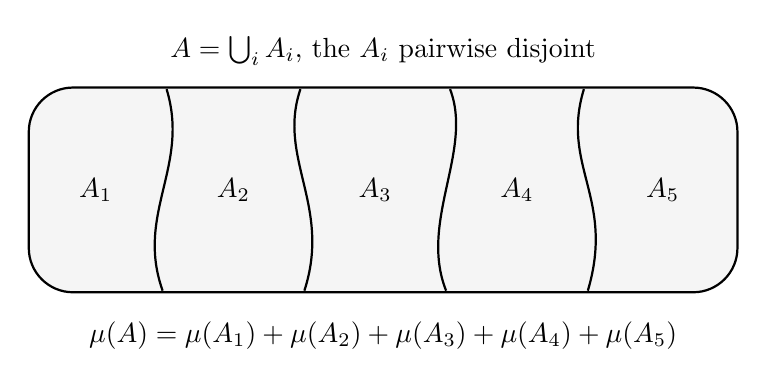
\begin{tikzpicture}[scale=1.0,>=stealth]
    \draw[thick,rounded corners=16pt,fill=gray!8] (0,0) rectangle (9,2.6);
    \draw[thick] (1.7,0.02) .. controls (1.35,1.0) and (2.05,1.6) .. (1.75,2.58);
    \draw[thick] (3.5,0.02) .. controls (3.85,1.1) and (3.15,1.7) .. (3.45,2.58);
    \draw[thick] (5.3,0.02) .. controls (4.95,0.9) and (5.65,1.8) .. (5.35,2.58);
    \draw[thick] (7.1,0.02) .. controls (7.45,1.2) and (6.75,1.6) .. (7.05,2.58);
    \node at (0.85,1.3) {$A_{1}$};
    \node at (2.6,1.3) {$A_{2}$};
    \node at (4.4,1.3) {$A_{3}$};
    \node at (6.2,1.3) {$A_{4}$};
    \node at (8.05,1.3) {$A_{5}$};
    \node[above] at (4.5,2.75) {$A = \bigcup_{i} A_{i}$, the $A_{i}$ pairwise disjoint};
    \node[below] at (4.5,-0.25)
      {$\mu(A) = \mu(A_{1}) + \mu(A_{2}) + \mu(A_{3}) + \mu(A_{4}) + \mu(A_{5})$};
  \end{tikzpicture}
\end{figure}

\medskip
On notera que la mesure d'un ensemble est une quantité positive, éventuellement
infinie; $[0,+\infty]$, not $[0,+\infty[$, is the target on purpose. Une mesure
$\mu$ est dite \emph{finie} si $\mu(\Omega) < \infty$. Additivity is required for
countable families and not merely finite ones, and only for \emph{pairwise disjoint}
sets --- weakening either restriction breaks the theory.

\begin{example}[Mesure de comptage]
  Soit $\Omega$ un ensemble. La fonction $\mu(A) = \operatorname{card}(A)$ est une
  mesure sur $(\Omega,\mathcal{P}(\Omega))$, appelée la \textbf{mesure de comptage}
  (\textit{counting measure}). It is finite exactly when $\Omega$ is finite.
\end{example}

\begin{example}[Mesure de Dirac]
  Soit $(\Omega,\mathcal{F})$ un espace mesurable et $a \in \Omega$. La fonction
  \[
    \delta_{a}(A) =
    \begin{cases}
      1 & \text{if } a \in A,\\
      0 & \text{otherwise,}
    \end{cases}
    \qquad A \in \mathcal{F},
  \]
  est une mesure, appelée la \textbf{mesure de Dirac} (\textit{Dirac measure}) en
  $a$. It is a mesure de probabilité: $\delta_{a}(\Omega) = 1$.
\end{example}

On vérifie facilement que toute somme au plus dénombrable de mesures est une
mesure: the check swaps two positive sums.

\begin{example}[Mesure de comptage de $\mathbb{N}$]
  La fonction $\mu = \sum_{n \in \mathbb{N}} \delta_{n}$ est une mesure sur
  $(\reals,\mathcal{B}(\reals))$: $\mu(A)$ counts the integers lying in $A$. Elle est
  appelée la mesure de comptage de $\mathbb{N}$, and it is the mesure with respect
  to which a sum over $\mathbb{N}$ will later be read as an integral.
\end{example}

\begin{definition}[Mesure $\sigma$-finie]
  Une mesure $\mu$ sur $(\Omega,\mathcal{F})$ est dite \textbf{$\sigma$-finie}
  (\textit{$\sigma$-finite}) si $\Omega$ peut être couvert par une réunion
  dénombrable d'ensembles de mesures finies.
\end{definition}

\begin{example}[$\sigma$-finite but not finite]
  La mesure de comptage de $\mathbb{N}$ sur $(\reals,\mathcal{B}(\reals))$ est
  $\sigma$-finie, en remarquant que $\reals = \bigcup_{n \geq 1} [-n,n]$ --- each
  $[-n,n]$ carries finitely many integers. Par contre, cette mesure n'est pas finie :
  $\mu(\reals) = +\infty$. The mesure de Lebesgue is $\sigma$-finie for the same
  covering, and also not finite.
\end{example}

$\sigma$-finiteness is the hypothesis that lets a statement about finite mesures be
transported to an infinite one by exhausting $\Omega$ along an increasing sequence.
It is close to, but weaker than, the covering hypothesis of the théorème d'unicité
below --- there the covering sets are required to lie in $\mathcal{C}$ itself --- and
it is a hypothesis of Fubini; when a result about mesures fails, the failure is
usually here.

\begin{prop}[Inclusion-exclusion et monotonie]
  Soit $\mu$ une mesure sur $(\Omega,\mathcal{F})$. Pour tous $A, B \in \mathcal{F}$,
  \begin{enumerate}
    \item $\mu(A \union B) + \mu(A \intersect B) = \mu(A) + \mu(B)$ ;
    \item si $A \subr B$, alors $\mu(A) \leq \mu(B)$.
  \end{enumerate}
\end{prop}

\begin{remark}
  Both come from $\sigma$-additivité applied to a decomposition into disjoint
  pieces. For the first, $A \union B = A \,\dunion\, (B \setminus A)$ gives
  $\mu(A \union B) + \mu(A \intersect B) = \mu(A) + \mu(B \setminus A) + \mu(A
  \intersect B) = \mu(A) + \mu(B)$, the last step because $B = (B \setminus A)
  \,\dunion\, (A \intersect B)$. For the second, $B = A \,\dunion\, (B
  \setminus A)$ and $\mu(B \setminus A) \geq 0$. Notice that the first identity is
  stated as a sum, not as $\mu(A \union B) = \mu(A) + \mu(B) - \mu(A \intersect B)$:
  the subtracted form is meaningless when $\mu(A \intersect B) = +\infty$. The
  additive form holds always.
\end{remark}

\subsubsection{Convergence monotone}

Une suite $(A_{n})_{n \geq 1}$ d'éléments de $\mathcal{F}$ est dite
\emph{croissante} si $A_{n} \subr A_{n+1}$ pour tout $n$ ; sa limite est alors $A =
\bigcup_{n} A_{n}$, ce que l'on notera $A_{n} \uparrow A$. De même, elle est dite
\emph{décroissante} si $A_{n+1} \subr A_{n}$ pour tout $n$ ; sa limite est $A =
\bigcap_{n} A_{n}$, ce que l'on notera $A_{n} \downarrow A$.

\begin{prop}[Continuité monotone, borne de l'union]
  Soit $\mu$ une mesure sur $(\Omega,\mathcal{F})$ et $(A_{n})_{n \geq 1}$ une suite
  d'éléments de $\mathcal{F}$.
  \begin{enumerate}
    \item Si $A_{n} \uparrow A$, alors $\mu(A) = \lim_{n} \uparrow \mu(A_{n})$.
    \item Si $A_{n} \downarrow A$ \textbf{et $\mu(A_{1}) < \infty$}, alors $\mu(A) =
      \lim_{n} \downarrow \mu(A_{n})$.
    \item On a la borne de l'union :
      $\displaystyle \mu\Bigl(\bigcup_{n \geq 1} A_{n}\Bigr) \leq \sum_{n \geq 1}
      \mu(A_{n})$, for any sequence, disjoint or not.
  \end{enumerate}
\end{prop}

\begin{remark}
  Continuity from below is $\sigma$-additivité in disguise: write $A = A_{1}
  \,\dunion\, (A_{2} \setminus A_{1}) \,\dunion\, \cdots$ and read the
  telescoping series as the limit of its partial sums. Continuity from above follows
  by passing to complements inside $A_{1}$, which is where the finiteness enters ---
  the step subtracts $\mu(A_{n})$ from $\mu(A_{1})$, and subtraction is not defined
  when both are $+\infty$. The borne de l'union follows from the disjointification
  $\bigcup_{n} A_{n} = \bigcup_{n} \bigl(A_{n} \setminus \bigcup_{k<n} A_{k}\bigr)$
  together with monotonicity.
\end{remark}

\begin{example}[Continuity from above fails without the finiteness hypothesis]
  Soit $\lambda$ la mesure de Lebesgue sur $\reals$ et $A_{n} = [n,+\infty[$ pour
  $n \geq 1$. The sequence is decreasing, and $\bigcap_{n \geq 1} A_{n} = \emptyset$,
  so $A_{n} \downarrow \emptyset$. Then
  \[
    \lambda\bigl(\lim_{n} \downarrow A_{n}\bigr) = \lambda(\emptyset) = 0,
    \qquad\text{whereas}\qquad
    \lim_{n} \downarrow \lambda(A_{n}) = +\infty,
  \]
  since $\lambda(A_{n}) = +\infty$ for every $n$. The two are not equal. The
  hypothesis $\mu(A_{1}) < \infty$ is violated --- $\lambda(A_{1}) = +\infty$ --- and
  the conclusion is false; the mass escapes to infinity rather than being destroyed.
  Dropping that one-line hypothesis is the classic error of the chapter, and this is
  the counter-example that catches it. Note that it is $\mu(A_{1})$, not $\mu(A)$,
  that must be finite: here $\mu(A) = 0$ and the conclusion still fails.
\end{example}

\subsubsection{Unicité}

Lorsque la tribu est engendrée par une collection d'ensembles (comme la tribu de
Borel, by the intervals), il est naturel de définir la mesure uniquement sur cette
collection d'ensembles, la mesure des autres ensembles s'en déduisant par
$\sigma$-additivité. Le \textbf{théorème d'unicité} (\textit{uniqueness theorem})
permet de formaliser cette idée.

\begin{theorem}[Unicité]
  Soit $\mu$ une mesure sur l'espace mesurable $(\Omega,\mathcal{F})$, avec
  $\mathcal{F} = \sigma(\mathcal{C})$ pour une certaine collection $\mathcal{C} \subr
  \mathcal{P}(\Omega)$. On suppose que :
  \begin{itemize}
    \item $\mathcal{C}$ est \textbf{stable par intersection finie}
      (\textit{stable under finite intersection}) --- a \emph{$\pi$-system} ---,
    \item $\Omega$ peut être couvert par une union dénombrable d'éléments de
      $\mathcal{C}$ de mesures finies.
  \end{itemize}
  S'il existe une mesure $\nu$ qui coïncide avec $\mu$ sur $\mathcal{C}$ alors $\nu
  = \mu$.
\end{theorem}

\begin{proof}
  Soit $B_{n} \uparrow \Omega$ une suite d'éléments de $\mathcal{C}$ telle que
  $\mu(B_{n}) < \infty$ pour tout $n \geq 1$ --- an increasing sequence, which is how
  the covering hypothesis is used: $\mathcal{C}$ is assumed stable par intersection
  finie only, so the finite unions of a bare cover need not lie in $\mathcal{C}$ and
  the cover is taken increasing from the start --- as it already is in every
  application below, $\reals = \bigcup_{n \geq 1} [-n,n]$ being the model. Pour tout
  $n$ fixé, soit
  \[
    \mathcal{M} = \{A \in \mathcal{F} : \mu(A \intersect B_{n}) = \nu(A \intersect
    B_{n})\}.
  \]
  On vérifie que $\mathcal{M}$ est une \textbf{classe monotone} (\textit{monotone
  class}) --- it contains $\Omega$, it is stable under proper difference, and it
  is stable under increasing limits. The lemme de classe monotone and the notion
  itself are carried in the reference chapter.
  \begin{itemize}
    \item $\Omega \in \mathcal{M}$: indeed $\Omega \intersect B_{n} = B_{n} \in
      \mathcal{C}$, where $\mu$ and $\nu$ agree by hypothesis.
    \item Si $A, B \in \mathcal{M}$ tels que $A \subr B$, alors
      \[
        \mu\bigl((B \setminus A) \intersect B_{n}\bigr)
        = \mu(B \intersect B_{n}) - \mu(A \intersect B_{n})
        = \nu(B \intersect B_{n}) - \nu(A \intersect B_{n})
        = \nu\bigl((B \setminus A) \intersect B_{n}\bigr),
      \]
      si bien que $B \setminus A \in \mathcal{M}$. \emph{The two subtractions are
      legal only because $\mu(A \intersect B_{n}) \leq \mu(B_{n}) < \infty$}, and the
      same for $\nu$; this is the single place where the finite-mesure half of the
      covering hypothesis is used, and without it the step is $\infty - \infty$.
    \item If $A_{1}, A_{2}, \ldots \in \mathcal{M}$ with $A_{k} \uparrow A$, then
      $A_{k} \intersect B_{n} \uparrow A \intersect B_{n}$ and continuity from below
      gives
      \[
        \mu(A \intersect B_{n}) = \lim_{k \to +\infty} \mu(A_{k} \intersect B_{n})
        = \lim_{k \to +\infty} \nu(A_{k} \intersect B_{n})
        = \nu(A \intersect B_{n}),
      \]
      si bien que $A \in \mathcal{M}$.
  \end{itemize}
  Next, $\mathcal{C} \subr \mathcal{M}$: for $A \in \mathcal{C}$ the set $A
  \intersect B_{n}$ again belongs to $\mathcal{C}$, \emph{because $\mathcal{C}$ is
  stable par intersection finie}, and $\mu$ and $\nu$ agree on $\mathcal{C}$.
  Hence the classe monotone generated by $\mathcal{C}$ satisfies $\mathcal{M}(
  \mathcal{C}) \subr \mathcal{M}$. Mais par le lemme de classe monotone --- whose own
  hypothesis is, once more, that $\mathcal{C}$ is stable par intersection finie
  ---, $\mathcal{M}(\mathcal{C}) = \sigma(\mathcal{C}) = \mathcal{F}$. On en déduit
  que $\mathcal{M} = \mathcal{F}$, de sorte que
  \[
    \forall A \in \mathcal{F}, \qquad \mu(A \intersect B_{n}) = \nu(A \intersect
    B_{n}).
  \]
  Finally let $n \to +\infty$. Since $A \intersect B_{n} \uparrow A$, continuity from
  below gives $\mu(A) = \nu(A)$ pour tout $A \in \mathcal{F}$, ce qui signifie que
  $\mu = \nu$.
\end{proof}

\begin{remark}[Where each hypothesis is spent]
  Stability of $\mathcal{C}$ under finite intersection is used twice, and both uses
  are essential: once to know that $A \intersect B_{n}$ is still a set on which $\mu$
  and $\nu$ are known to agree, and once inside the lemme de classe monotone, which
  is false without it. The finite-mesure covering is used twice as well: to make the
  difference step a legal subtraction, and to exhaust $\Omega$ at the end. Two
  mesures agreeing on a generating family that is \emph{not} a $\pi$-system may
  differ --- the theorem is not a formality, and on an exam the first thing to check
  is that the collection offered is closed under intersection.
\end{remark}

\subsubsection{Mesure de Lebesgue}

\begin{definition}[Mesure de Lebesgue sur $\reals$]
  La mesure de Lebesgue sur $(\reals,\mathcal{B}(\reals))$ est l'unique mesure,
  notée $\lambda$, telle que pour tous réels $a < b$,
  \[
    \lambda([a,b]) = b - a.
  \]
\end{definition}

La preuve de l'existence d'une telle mesure est difficile: it is obtained by
building an outer mesure from countable coverings by intervals, showing that the
sets splitting every test set additively form a tribu containing the boréliens, and
restricting. L'unicité est une conséquence directe du théorème d'unicité. Il suffit
en effet de considérer la collection $\mathcal{C}$ des intervalles $[a,b]$ avec $a
\leq b$, complétée de $\emptyset$. Cette collection est stable par intersection
finie, since the intersection of two such intervals is again one or is empty, and
$\reals = \bigcup_{n \geq 1} [-n,n]$ is a countable cover by elements of finite
mesure. Toute autre mesure $\nu$ qui donne la mesure $b - a$ à l'intervalle $[a,b]$
est nécessairement égale à $\lambda$.

\begin{remark}[Three consequences, each a one-line computation]
  Pour tout $a \in \reals$, $\lambda(\{a\}) = 0$, en utilisant le fait que $\{a\} =
  \bigcap_{n \geq 1} [a - \tfrac{1}{n}, a + \tfrac{1}{n}]$ --- a decreasing limit
  with $\lambda([a-1,a+1]) = 2 < \infty$, so continuity from above applies and gives
  $\lim_{n} \tfrac{2}{n} = 0$. Then $\lambda(\mathbb{Q}) = 0$ par
  $\sigma$-additivité, $\mathbb{Q}$ being a countable union of singletons. And
  $\lambda(\reals \setminus \mathbb{Q}) = +\infty$, since
  $\lambda(\reals) = \lambda(\mathbb{Q}) + \lambda(\reals \setminus \mathbb{Q})$ and
  $\lambda(\reals) = +\infty$. A countable set is invisible to $\lambda$; an
  uncountable one need not be visible either, as the ensemble de Cantor shows below.
\end{remark}

\begin{prop}[Invariance par translation (\textit{translation invariance})]
  Pour tout borélien $A$ et tout $t \in \reals$, $\lambda(A + t) = \lambda(A)$.
\end{prop}

\begin{remark}
  First, $A + t$ is a borélien whenever $A$ is: $\{B - t : B \in
  \mathcal{B}(\reals)\}$ is a tribu containing the intervals, hence contains
  $\mathcal{B}(\reals)$. So $\lambda(A+t)$ is defined. Notons $\mu(A) =
  \lambda(A+t)$ pour $A \in \mathcal{B}(\reals)$. On vérifie que
  $\mu$ est une mesure --- translation preserves disjointness and countable unions
  --- and $\mu([a,b]) = \lambda([a+t,b+t]) = b-a$, so $\mu$ coïncide avec $\lambda$
  sur les intervalles. D'après le théorème d'unicité, $\mu = \lambda$. This is the
  standard use of the theorem: to identify two mesures, check them on a
  $\pi$-system and stop. Conversely, la mesure de Lebesgue est la \emph{seule}
  mesure $\sigma$-finie invariante par translation sur $(\reals,\mathcal{B}(\reals))$,
  à une constante multiplicative près; the constant is recovered as $\alpha =
  \mu([0,1[)$, which is finite precisely because $\mu$ is $\sigma$-finie, and one
  then propagates $\mu([0,x[) = \alpha x$ from $x \in \mathbb{N}$ to $x \in
  \mathbb{Q}_{+}$ and finally to $x \in \reals_{+}$ by monotone limits.
\end{remark}

\begin{definition}[Mesure de Lebesgue sur $\reals^{n}$]
  La mesure de Lebesgue sur $(\reals^{n},\mathcal{B}(\reals^{n}))$ est l'unique
  mesure, que l'on notera également $\lambda$, telle que pour tous réels $a_{1} <
  b_{1}, \ldots, a_{n} < b_{n}$,
  \[
    \lambda\bigl([a_{1},b_{1}] \times \cdots \times [a_{n},b_{n}]\bigr)
    = (b_{1}-a_{1}) \cdots (b_{n}-a_{n}).
  \]
\end{definition}

Cette mesure est également la seule mesure $\sigma$-finie invariante par translation
sur $\reals^{n}$, à une constante multiplicative près. The $\sigma$-finiteness is
not decoration: without it the characterisation is false, and it is what a
computation of the image of $\lambda$ under an invertible affine map has to check
first.

\begin{example}[A mesure that is neither Lebesgue nor atomic]
  On $(\reals,\mathcal{B}(\reals))$ put $\mu = \lambda + \delta_{0}$, a sum of two
  mesures and therefore a mesure. Then
  \[
    \mu(\{0\}) = 1, \quad \mu([0,1]) = 2, \quad \mu([-1,1]) = 3, \quad
    \mu([-1,0[) = 1, \quad \mu(\reals_{+}) = +\infty.
  \]
  Each is the Lebesgue length plus $1$ if $0$ is in the set. In $\reals^{2}$ with
  $\mu = \lambda + \delta_{(0,0)}$ the same reading gives $\mu(\{(0,0)\}) = 1$,
  $\mu([0,1]^{2}) = 2$, $\mu([-1,1]^{2}) = 5$, $\mu([-1,0[^{2}) = 1$ and
  $\mu(\reals_{+} \times \{0\}) = 1$, the last because that half-line has mesure de
  Lebesgue zero in the plane and contains the origin.
\end{example}

\subsection{Ensembles négligeables}

Soit $\mu$ une mesure sur $(\Omega,\mathcal{F})$.

\begin{definition}[Ensemble négligeable]
  Un ensemble $A \in \mathcal{F}$ est dit \textbf{négligeable} (\textit{negligible})
  si $\mu(A) = 0$.
\end{definition}

Une propriété est dite vraie \textbf{presque partout} (\textit{almost everywhere})
si sa négation correspond à un ensemble négligeable. The abbreviation p.p. is kept
in its French form, and it is the primary form in these notes; the mesure it refers
to is always named or clear from the context.

\begin{example}[Almost every real is irrational]
  Presque tout réel est irrationnel pour la mesure de Lebesgue: $\lambda(\mathbb{Q})
  = 0$, so the set of rationals is négligeable. There are as many rationals as
  integers and uncountably many reals, and $\lambda$ sees only the second fact.
\end{example}

\begin{remark}[Negligible with respect to which mesure?]
  Negligibility is a statement about a pair, a set \emph{and} a mesure: il faut
  veiller à bien spécifier la mesure considérée. Par exemple, il est faux de dire
  que presque tout réel est irrationnel pour la mesure $\mu = \lambda + \delta_{0}$:
  $\mu(\mathbb{Q}) \geq \mu(\{0\}) = 1 \neq 0$, so $\mathbb{Q}$ n'est pas
  négligeable pour $\mu$, even though it is for $\lambda$. Two mesures on the same
  tribu can disagree completely about which sets are négligeables.
\end{remark}

\begin{example}[An uncountable negligible set: the ensemble de Cantor]
  Let $C_{0} = [0,1[$, and let $C_{n+1}$ be obtained from $C_{n}$ by deleting the
  open middle third of each of its intervals, so that
  \[
    C_{1} = \Bigl[0,\tfrac{1}{3}\Bigr[ \,\union\, \Bigl[\tfrac{2}{3},1\Bigr[,
    \qquad
    C_{2} = \Bigl[0,\tfrac{1}{9}\Bigr[ \,\union\, \Bigl[\tfrac{2}{9},\tfrac{1}{3}
    \Bigr[ \,\union\, \Bigl[\tfrac{2}{3},\tfrac{7}{9}\Bigr[ \,\union\,
    \Bigl[\tfrac{8}{9},1\Bigr[,
  \]
  and set $C = \bigcap_{n \geq 0} C_{n}$, the \textbf{ensemble de Cantor}
  (\textit{Cantor set}). A real of $[0,1[$ lies in $C_{n}$ exactly when none of
  the first $n$ digits of its ternary expansion is $1$, so $C$ is the set of reals whose
  ternary expansion uses only the digits $0$ and $2$. Replacing every $2$ by a $1$
  maps $C$ bijectively onto the binary expansions, that is onto $[0,1[$: the
  ensemble de Cantor is uncountable. Yet $C_{n}$ is a union of $2^{n}$ intervals of
  length $3^{-n}$, so $\lambda(C_{n}) = (2/3)^{n}$, and $C_{n} \downarrow C$ with
  $\lambda(C_{0}) = 1 < \infty$, so continuity from above applies and
  \[
    \lambda(C) = \lim_{n} \left(\frac{2}{3}\right)^{n} = 0 .
  \]
  Being négligeable is therefore not a statement about cardinality. Note that the
  finiteness hypothesis was available here and had to be invoked.
\end{example}

\subsection{Fonctions mesurables}

Soit $(\Omega,\mathcal{F})$ et $(E,\mathcal{E})$ deux espaces mesurables.

\begin{definition}[Fonction mesurable]
  Une fonction $f : \Omega \to E$ est dite \textbf{mesurable} (\textit{measurable})
  si :
  \[
    \forall A \in \mathcal{E}, \qquad f^{-1}(A) \in \mathcal{F}.
  \]
\end{definition}

\begin{figure}[h!]
  \centering
  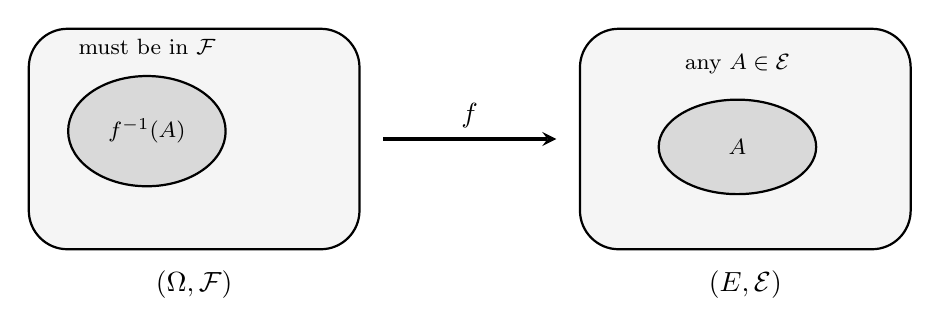
\begin{tikzpicture}[scale=1.0,>=stealth]
    \draw[thick,rounded corners=14pt,fill=gray!8] (0,0) rectangle (4.2,2.8);
    \draw[thick,rounded corners=14pt,fill=gray!8] (7.0,0) rectangle (11.2,2.8);
    \node[below] at (2.1,-0.15) {$(\Omega,\mathcal{F})$};
    \node[below] at (9.1,-0.15) {$(E,\mathcal{E})$};
    \draw[thick,fill=gray!30] (1.5,1.5) ellipse (1.0 and 0.7);
    \draw[thick,fill=gray!30] (9.0,1.3) ellipse (1.0 and 0.6);
    \node at (1.5,1.5) {\footnotesize $f^{-1}(A)$};
    \node at (9.0,1.3) {\footnotesize $A$};
    \draw[->,very thick] (4.5,1.4) -- (6.7,1.4) node[midway,above] {$f$};
    \node[above] at (1.5,2.35) {\footnotesize must be in $\mathcal{F}$};
    \node[above] at (9.0,2.1) {\footnotesize any $A \in \mathcal{E}$};
  \end{tikzpicture}
\end{figure}

\medskip
Measurability is a condition on \emph{preimages}, never on images, because $f^{-1}$
commutes with every set operation --- complement, arbitrary union, arbitrary
intersection --- while the direct image does not commute with complement. That one
algebraic fact makes the whole of this subsection work.

\begin{example}[The indicator function is measurable]
  Soit $A \in \mathcal{F}$. La fonction $f = \indic_{A}$ est mesurable de
  $(\Omega,\mathcal{F})$ vers $(\reals,\mathcal{B}(\reals))$. En effet, pour tout
  borélien $B$,
  \[
    f^{-1}(B) =
    \begin{cases}
      A & \text{if } 1 \in B, \; 0 \notin B,\\
      A^{c} & \text{if } 1 \notin B, \; 0 \in B,\\
      \Omega & \text{if } 0, 1 \in B,\\
      \emptyset & \text{if } 0, 1 \notin B,
    \end{cases}
  \]
  and all four are in $\mathcal{F}$. Only four preimages occur because $f$ takes only
  two values; measurability of $\indic_{A}$ is exactly the statement $A \in
  \mathcal{F}$.
\end{example}

\begin{remark}
  On remarque que si $\mathcal{F} = \mathcal{P}(\Omega)$ alors toute fonction sur
  $\Omega$ est mesurable, whatever the target. Measurability constrains only when the
  source tribu is genuinely smaller than the ensemble des parties: it measures how
  much information $\mathcal{F}$ carries about $f$.
\end{remark}

\begin{lemma}[La mesurabilité se vérifie sur une collection génératrice]
  Soit $\mathcal{C} \subr \mathcal{P}(E)$ une collection d'ensembles telle que
  $\mathcal{E} = \sigma(\mathcal{C})$. Une condition suffisante pour que $f : \Omega
  \to E$ soit mesurable est que :
  \[
    \forall A \in \mathcal{C}, \qquad f^{-1}(A) \in \mathcal{F}.
  \]
\end{lemma}

\begin{remark}
  Soit $\mathcal{G} = \{A \in \mathcal{E} : f^{-1}(A) \in \mathcal{F}\}$. It is a
  tribu, precisely because $f^{-1}$ commutes with complement and countable union:
  $f^{-1}(E) = \Omega$, $f^{-1}(A^{c}) = f^{-1}(A)^{c}$ and $f^{-1}(\bigcup_{i}
  A_{i}) = \bigcup_{i} f^{-1}(A_{i})$. Par hypothèse, $\mathcal{C} \subr
  \mathcal{G}$, donc $\mathcal{E} = \sigma(\mathcal{C}) \subr \mathcal{G}$, ce qui
  signifie que la fonction $f$ est mesurable. This lemma is the workhorse of the
  subsection: every measurability proof below applies it to a well-chosen generating
  family, and for a real-valued function that family is almost always the half-lines
  $]-\infty,b]$.
\end{remark}

\subsubsection{Mesure image}

Si $\mu$ est une mesure sur $(\Omega,\mathcal{F})$, toute fonction mesurable définit
une nouvelle mesure, transported to the target.

\begin{definition}[Mesure image]
  Soit $f : \Omega \to E$ une fonction mesurable. La mesure $\mu_{f}$ définie par :
  \[
    \forall A \in \mathcal{E}, \qquad \mu_{f}(A) = \mu\bigl(f^{-1}(A)\bigr)
  \]
  est appelée la \textbf{mesure image} (\textit{image measure}) de $\mu$ par $f$.
\end{definition}

That $\mu_{f}$ is a mesure is again the commutation of $f^{-1}$ with the set
operations: preimages of disjoint sets are disjoint, and a countable disjoint union
pulls back to one. This construction later carries the whole of probability --- the
loi of a variable aléatoire is the image of $\prob$ by that variable, and nothing
else.

\begin{example}[Mesure image sur un espace à deux points]
  Soit $\Omega = \{1,2,3\}$ et $\mu$ la mesure de comptage sur
  $(\Omega,\mathcal{P}(\Omega))$, and $f = \indic_{\{1,2\}}$ with values in $E =
  \{0,1\}$. Then $f^{-1}(\{0\}) = \{3\}$ and $f^{-1}(\{1\}) = \{1,2\}$, so
  \[
    \mu_{f}(\{0\}) = 1, \qquad \mu_{f}(\{1\}) = 2 .
  \]
  The total mass $3$ is preserved: a mesure image never creates or destroys mass,
  it only redistributes it.
\end{example}

\begin{example}[Mesure de Lebesgue et fonction affine]
  Soit $\phi : \reals \to \reals$ la fonction affine $\phi(x) = \alpha x + \beta$,
  avec \textbf{$\alpha \neq 0$}. Pour $a < b$,
  \[
    x \in \phi^{-1}([a,b])
    \iff a \leq \alpha x + \beta \leq b,
  \]
  on obtient l'intervalle $\bigl[\tfrac{a-\beta}{\alpha}, \tfrac{b-\beta}{\alpha}
  \bigr]$ si $\alpha > 0$ et l'intervalle $\bigl[\tfrac{b-\beta}{\alpha},
  \tfrac{a-\beta}{\alpha}\bigr]$ si $\alpha < 0$; in both cases its length is
  $(b-a)/|\alpha|$. On en déduit $\lambda_{\phi}([a,b]) = (b-a)/|\alpha|$, and the
  two mesures $\lambda_{\phi}$ and $\lambda/|\alpha|$ agree on the intervals, a
  $\pi$-system generating $\mathcal{B}(\reals)$ along a countable cover of finite
  mesure. By the théorème d'unicité,
  \[
    \lambda_{\phi} = \frac{\lambda}{|\alpha|} .
  \]
  The invertibility $\alpha \neq 0$ is essential: for $\alpha = 0$ the map is
  constant, the
  preimage of a set is $\emptyset$ or $\reals$, and the mesure image is not even
  $\sigma$-finie. In $\reals^{n}$ the same statement holds for $\phi(x) = Ax + b$
  with $A$ \textbf{invertible}, and reads $\lambda_{\phi} = \lambda/|\det A|$;
  the proof reduces the general case to the diagonal, orthogonal and symmetric ones
  through the polar decomposition $A = QS$, and the first step is precisely the
  check that $\lambda_{\phi}$ is $\sigma$-finie and translation-invariant.
\end{example}

\subsubsection{Stabilité de la mesurabilité}

\begin{prop}[Composition de fonctions]
  Soit $(G,\mathcal{G})$ un espace mesurable. Si les fonctions $f : \Omega \to E$ et
  $g : E \to G$ sont mesurables, la fonction $g \circ f : \Omega \to G$ est
  mesurable.
\end{prop}

\begin{remark}
  One line: pour tout ensemble $A \in \mathcal{G}$, on a $g^{-1}(A) \in \mathcal{E}$
  because $g$ is mesurable, donc $f^{-1}\bigl(g^{-1}(A)\bigr) \in \mathcal{F}$ because
  $f$ is; and $(g \circ f)^{-1}(A) = f^{-1}(g^{-1}(A))$.
\end{remark}

On s'intéresse maintenant aux fonctions réelles $f : \Omega \to \reals$ ou
vectorielles $f : \Omega \to \reals^{n}$, les ensembles $\reals$ et $\reals^{n}$
étant munis de leur tribu de Borel.

\begin{prop}[Continuité implique mesurabilité]
  Toute fonction continue $f : \Omega \to \reals^{n}$, avec $\Omega = \reals$ ou
  $\reals^{m}$ muni de sa tribu de Borel, est mesurable.
\end{prop}

\begin{remark}
  Under a continuous map, l'image réciproque d'un ouvert est un ouvert, hence a
  borélien; la tribu de Borel de $\reals^{n}$ étant engendrée par les ouverts,
  conclude by the generating lemma. This is the one place where the characterisation
  of $\mathcal{B}(\reals)$ by the open sets, rather than by the intervals, is what
  makes the argument work at all.
\end{remark}

\begin{remark}[The converse is false]
  Il existe des fonctions mesurables qui ne sont pas continues. Par exemple, la
  fonction $\indic_{\mathbb{Q}} : \reals \to \reals$ est mesurable puisque
  $\mathbb{Q}$ est un borélien, and is continuous at no point. Measurability is much
  weaker than continuity, and that weakness is the point: the class of mesurable
  functions is closed under operations --- limits above all --- under which the
  continuous functions are not.
\end{remark}

\begin{prop}[Mesurabilité coordonnée par coordonnée]
  Soit $f = (f_{1},\ldots,f_{n})$ une fonction de $\Omega$ vers $\reals^{n}$. La
  fonction $f$ est mesurable si et seulement si les fonctions $f_{1},\ldots,f_{n}$
  sont mesurables.
\end{prop}

\begin{remark}
  Forwards: $f_{1}^{-1}([a,b]) = f^{-1}([a,b] \times \reals \times \cdots \times
  \reals)$, a preimage of a borélien, so $f_{1}$ is mesurable by the generating
  lemma, and likewise for the other coordinates. Réciproquement, pour tout pavé,
  \[
    f^{-1}\bigl([a_{1},b_{1}] \times \cdots \times [a_{n},b_{n}]\bigr)
    = f_{1}^{-1}([a_{1},b_{1}]) \intersect \cdots \intersect
      f_{n}^{-1}([a_{n},b_{n}]),
  \]
  a finite intersection of elements of $\mathcal{F}$; the pavés generate
  $\mathcal{B}(\reals^{n})$, so the generating lemma applies again.
\end{remark}

\begin{prop}[Opérations algébriques]
  Si $f$ et $g$ sont des fonctions mesurables, alors les fonctions $f + g$, $fg$,
  $\max(f,g)$ et $\min(f,g)$ sont mesurables.
\end{prop}

\begin{remark}
  Each is a composition. La fonction addition $\reals^{2} \to \reals$, $(x,y) \mapsto
  x + y$, est continue donc mesurable; the pair $(f,g) : \Omega \to \reals^{2}$ is
  mesurable by coordinatewise measurability; so $f + g$ is mesurable as a
  composition of two mesurable maps. Multiplication, $\max$ and $\min$ are
  continuous in the same way: la preuve est identique pour les autres opérations.
  Note the order of the three propositions: composition, then coordinates, then
  operations --- each uses the one before.
\end{remark}

\begin{example}[Fonction mesurable sur $\reals$]
  La fonction $f(x) = x^{2} + \indic_{\reals_{+}}(x)$ est mesurable de
  $(\reals,\mathcal{B}(\reals))$ vers $(\reals,\mathcal{B}(\reals))$ : c'est la somme
  de deux fonctions mesurables, la fonction continue $x \mapsto x^{2}$, mesurable
  because continuous, et la fonction indicatrice du borélien $\reals_{+}$, mesurable
  because $\reals_{+}$ is a borélien. It is discontinuous at $0$, which costs nothing.
\end{example}

\begin{example}[Fonction mesurable sur $\reals^{2}$]
  Likewise, la fonction $f(x,y) = xy + \indic_{\{(0,0)\}}(x,y)$ est mesurable de
  $(\reals^{2},\mathcal{B}(\reals^{2}))$ vers $(\reals,\mathcal{B}(\reals))$ : c'est
  la somme de deux fonctions mesurables, la fonction continue $(x,y) \mapsto xy$ et
  la fonction indicatrice du singleton $\{(0,0)\}$, which is a borélien of
  $\reals^{2}$.
\end{example}

\subsubsection{Limites de fonctions mesurables}

Here the class of mesurable functions shows what it is for. Nous allons maintenant
considérer la limite d'une suite de fonctions mesurables, lorsqu'elle existe, et
montrer qu'on obtient une fonction mesurable. C'est une différence notable avec les
fonctions continues, la limite de fonctions continues n'étant pas continue en
général. Nous allons travailler sur l'ensemble $\bar{\reals}$, muni de sa tribu de
Borel $\mathcal{B}(\bar{\reals})$, since a supremum of real functions need not be
finite.

\begin{prop}[Supremum, infimum et limites]
  Soit $(f_{n})_{n \geq 1}$ une suite de fonctions mesurables de $\Omega$ vers
  $\bar{\reals}$. Alors les fonctions $\inf_{n} f_{n}$, $\sup_{n} f_{n}$,
  $\liminf_{n} f_{n}$, $\limsup_{n} f_{n}$ et $\lim_{n} f_{n}$ (lorsque celle-ci
  existe) sont des fonctions mesurables de $\Omega$ vers $\bar{\reals}$.
\end{prop}

\begin{remark}
  Soit $f = \sup_{n} f_{n}$. On a pour tout $b \in \bar{\reals}$ :
  \[
    f^{-1}\bigl([-\infty,b]\bigr) = \bigcap_{n \geq 1} f_{n}^{-1}
    \bigl([-\infty,b]\bigr) \in \mathcal{F},
  \]
  because $\sup_{n} f_{n}(\omega) \leq b$ if and only if $f_{n}(\omega) \leq b$ for
  every $n$. Comme $\mathcal{B}(\bar{\reals})$ est engendrée par les intervalles
  $[-\infty,b]$, la fonction $f$ est mesurable by the generating lemma. On montre de
  la même manière que l'infimum est mesurable, $\mathcal{B}(\bar{\reals})$ étant
  également engendrée par les intervalles $[a,+\infty]$. Then
  \[
    \liminf_{n} f_{n} = \sup_{n} \inf_{k \geq n} f_{k},
    \qquad
    \limsup_{n} f_{n} = \inf_{n} \sup_{k \geq n} f_{k},
  \]
  so both are mesurables by two applications of what precedes. Enfin, si la limite
  $\lim_{n} f_{n}$ est bien définie, elle vaut $\liminf_{n} f_{n}$, which settles it.
\end{remark}

\begin{remark}[Where $\bar{\reals}$ was needed]
  Nothing forces the sequence to be bounded, so $\sup_{n} f_{n}$ may legitimately be
  $+\infty$ on a set of positive mesure. Had the target been $\reals$, the
  proposition would have needed a boundedness hypothesis and would have been useless
  for the next chapter's théorème de convergence monotone and lemme de Fatou, both
  stated for positive mesurable functions with values in $[0,+\infty]$. This is why
  $\mathcal{B}(\bar{\reals})$ was defined at all.
\end{remark}

\begin{conclusion}
  The chapter fixes three objects and one theorem. The objects: a \emph{tribu}, which
  is the family of sets one is allowed to measure, generated in practice from a small
  collection --- intervals, half-lines, open sets, pavés --- rather than written out;
  a \emph{mesure}, a $\sigma$-additive map into $[0,+\infty]$, of which $\lambda$ and
  $\delta_{a}$ are the two models and all the rest are built from them; and a
  \emph{mesurable function}, defined by its preimages and therefore stable under
  composition, algebraic operations and, decisively, pointwise limits. The theorem is
  uniqueness: two mesures agreeing on a $\pi$-system that generates the tribu, with
  a countable cover of $\Omega$ by elements of that $\pi$-system of finite mesure,
  are equal --- which is what allows every later
  identification of a loi to stop after checking a generating family.\\

  Two hypotheses go missing under compression, and both were written out above:
  continuity from above needs $\mu(A_{1}) < \infty$, with $A_{n} = [n,+\infty[$ as
  the standing counter-example, and the théorème d'unicité needs $\mathcal{C}$ stable
  par intersection finie, used once to keep $A \intersect B_{n}$ inside
  $\mathcal{C}$ and once inside the lemme de classe monotone. The next chapter builds
  the integral on these objects, starting with positive mesurable functions valued in
  $[0,+\infty]$ --- the reason $\mathcal{B}(\bar{\reals})$ was defined here.
\end{conclusion}
